“You just stepped in the wrong pile of shit, cultist.”\\

Two armed men dressed in colorful leathers await your arrival in the barracks. They stand amongst three rows of blood-soaked cots, their sheets incarnadined by a host of slit throats--guards slaughtered in their smallclothes.\\

One of the men hefts a two-handed sword over his shoulder. The other tucks himself behind a round shield emblazoned with the emblem of a golden hand. Despite your common foe, it appears that these men--whoever they are--are no friends of the Black and Golden Key.\\

“Gentlemen...”\\

A woman reclines on a mattress propped up against an overturned chair. She lays clutching her side, where a dark red stain has spread across her dress of glittering sequins.\\

“Dispatch this interloper, and make haste. For I know not how much longer my strength will last me...”\\

“And let the glitter of gold guide you!”\\
She raises an ornate catalyst overhead, filling the barracks with a light both painful and blinding in its brilliance.\\

Your eyes soon adjust to find two silhouettes picking their way around the smashed cots and crumpled bodies, their forms made stark and ominous in the brassy halation.\\

\subsection*{Victory Condition}
Defeat all enemies

\subsection*{Doom Events}
\begin{itemize}
\item \textbf{Round 3:} \emph{The sorceress sputters, and coughs up a handful of blood.} Do not roll on Table C for this Round.
\item \textbf{Round 5:} \emph{The injured sorceress is wracked by convulsions.} Do not roll on Table C for this Round.
\item \textbf{Round 7:} \emph{The sorceress collapses against her mattress with a rattling gasp.} Lustrous Nastya is defeated, remove her token.
\end{itemize}

\pagebreak

\subsection*{Encounter Tables}
\begin{tcolorbox}
\textbf{Table A - Lustrous Nastya}
\begin{center}
\begin{tabular}{ L | L }
\multicolumn{1}{c|}{\textbf{1-3}} & 
\multicolumn{1}{c}{\textbf{4-6}} \\
\textbf{A:} \emph{Gilding}\newline \textbf{B:} \emph{Dazzle}\newline \textbf{C:} \emph{Greedy Endurance}\newline \emph{This result is only exhausted after its second token} &
\textbf{A:} \emph{Gilding}\newline \textbf{B:} \emph{Golden Arrow}\newline \textbf{C:} \emph{Clinking Motivation}\newline \emph{This result is only exhausted after its second token} \\
\end{tabular}
\end{center}
\textbf{Note:} If \emph{Gilding} is already in effect, Nastya will not cast it again (resolve the next behavior).
\end{tcolorbox}

\begin{tcolorbox}
\textbf{Table B - Goldhand Vitalik}
\begin{center}
\begin{tabular}{ L | L | L }
\multicolumn{1}{c|}{\textbf{1}} & 
\multicolumn{1}{c|}{\textbf{2-5}} & 
\multicolumn{1}{c}{\textbf{6}} \\
\textbf{A:} \emph{Sudden. Hidden Seax}\newline \textbf{B:} \emph{Shield Up!} Move &
\textbf{A:} \emph{Shield Up!} Move\newline \textbf{B:} Move. \emph{Guarded Mace}\newline \emph{This result is only exhausted after its third token} &
\textbf{A:} \emph{Bash}\newline \textbf{B:} Move. \emph{Guarded Mace} \\
\end{tabular}
\end{center}
\end{tcolorbox}

\begin{tcolorbox}
\textbf{Table C - Goldhand Sergey}
\begin{center}
\begin{tabular}{ L | L | L}
\multicolumn{1}{c|}{\textbf{1}} & 
\multicolumn{1}{c|}{\textbf{2-5}} &
\multicolumn{1}{c}{\textbf{6}}\\
\textbf{A:} \emph{Lunge}\newline \textbf{B:} Move &
Move. \emph{Claymore}\newline \emph{This result is only exhausted after its third token} &
\emph{Huff \& Puff} \\
\end{tabular}
\end{center}
\end{tcolorbox}


\subsection*{Enemy Sheets}
\hrule
\ \\
{\large \textbf{Goldhand Vitalik}}\\\\
\begin{tabular}{s s s}
\textbf{HP:} 8 & \textbf{Move:} 3\\
\textbf{P.DEF:} 1 & \textbf{RES:} 1\\
\textbf{Shield Def:} 2 & \textbf{Shield Stab:} 5 & \textbf{Shield Dur:} 1\\
\end{tabular}\\

\emph{Intelligent:} This entity is human, or possesses a human-like intellect.\\

\emph{Round Shield:} When this entity blocks non-\emph{Magical} ranged damage, do not place it on the \emph{Shield Up!} token.\\

\textbf{Attacks:}
\begin{itemize}
\item \emph{Guarded Mace} -  Deal 2 Crush damage on an adjacent entity. Do not remove \emph{Shield Up!}
\item \emph{Bash} - Deal 1 Crush damage and inflict Stun on an adjacent entity.
\item \emph{Hidden Seax} - Move 1. Deal 2 Slash damage. If any such damage is assigned to \textbf{HP} slots, inflict Bleeding.
\end{itemize}

\pagebreak

{\large \textbf{Goldhand Sergey}}\\\\
\begin{tabular}{s s s}
\textbf{HP:} 10 & \textbf{Move:} 3\\
\textbf{P.DEF:} 1 & \textbf{RES:} 2 & \textbf{PS:} 1\\
\end{tabular}\\

\emph{Intelligent:} This entity is human, or possesses a human-like intellect.\\

\textbf{Attacks:}
\begin{itemize}
\item \emph{Claymore} -  Deal 3 Slash damage to an adjacent entity.
\item \emph{Lunge} - Move 2. Deal 2 \emph{Unparryable} Pierce ranged melee damage to an entity within 2 hexes.
\item \emph{Wild Swing} - Move 2. Deal 4 \emph{Unparryable} Slash damage, Knockback 2, and Knockdown to \emph{all} hexes in a half-moon pattern centered on an adjacent entity.
\item \emph{Huff \& Puff} - No effect.
\end{itemize}
\hrule
\ \\
{\large \textbf{Lustrous Nastya}}\\\\
\begin{tabular}{s s s}
\textbf{HP:} 4 & \textbf{Move:} 0\\
\textbf{M.DEF:} 2 & \textbf{F.DEF:} 2 & \textbf{D.DEF:} 1\\
\end{tabular}\\

\emph{Intelligent:} This entity is human, or possesses a human-like intellect.\\

\emph{Profuse Bleeding:} This entity is immune to Bleeding and Bleed damage.\\

\textbf{Attacks:}
\begin{itemize}
\item \emph{Golden Arrow} -  Deal 1 \emph{Lock-On} Magic ranged damage to an entity within 4 hexes.
\item \emph{Dazzle} - Inflict Stun on an enemy within 2-3 hexes.
\item \emph{Gilding} - Add 1 Enhanced Defense: \textbf{P.DEF} (3) and 1 Enhanced Defense: \textbf{M.DEF} (1) condition token to Lustrous Nastya’s enemy sheet.
\item \emph{Clinking Motivation} - For this Turn, Goldhand Sergey’s \emph{Huff \& Puff} attack is replaced by \emph{Wild Swing}.
\item \emph{Greedy Endurance} - Clear Goldhand Vitalik’s \textbf{P.DEF} and \textbf{Shield Stab} of all damage tokens. 
\end{itemize}

\pagebreak

\subsection*{Encounter Map}
\begin{center}
\framebox{
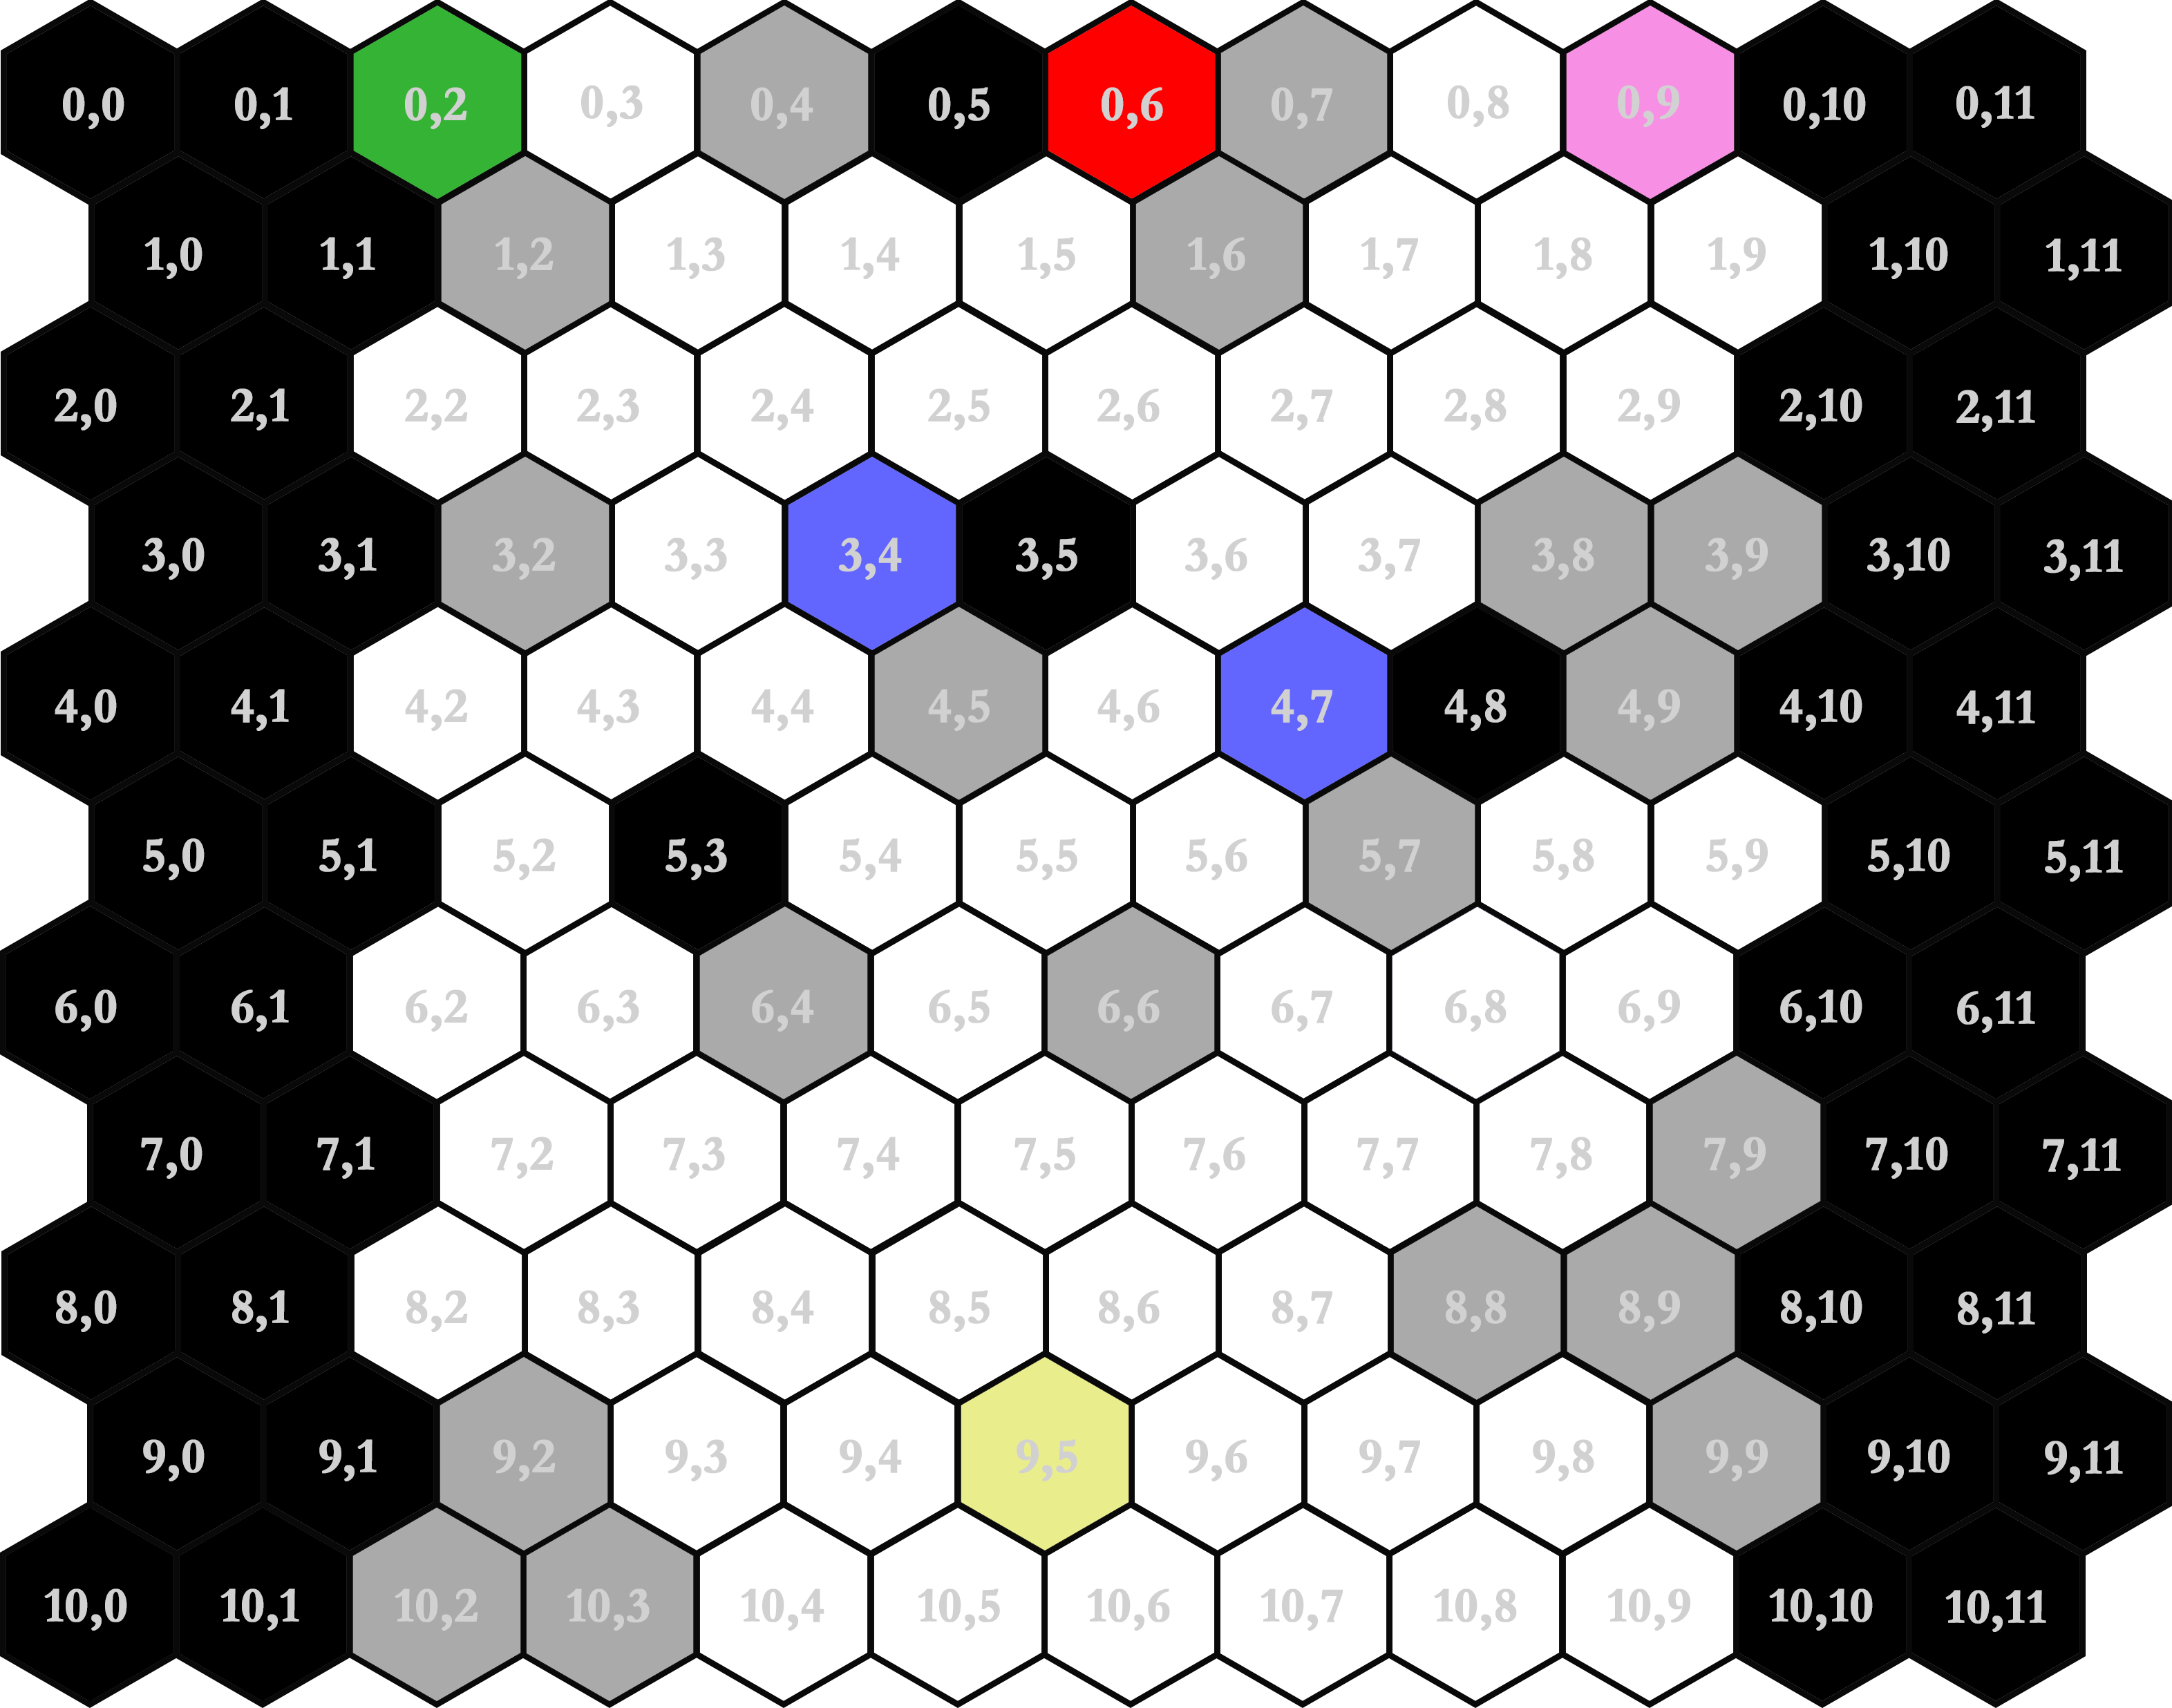
\includegraphics[width = 0.96\textwidth]{./maps/c311.png}
}
\end{center}

\subsection*{Setup Instructions}
\begin{itemize}
\item \textbf{Goldenrod:} Character Start Location.
\item \textbf{Pink:} Alternative Character Start Location. If the character entered c311 via climbing the rope from c327x1, place their token here.
\item \textbf{Red:} Enemy Start Location. Place Lustrous Nastya here.
\item \textbf{Blue:} Enemy Start Location. Place the Goldhands on either tile.
\item \textbf{Black:} Impassable Boundary/Full-Cover
\item \textbf{Light Gray:} Half-Cover.
\item \textbf{Green:} Escape Tile.
\end{itemize}

\pagebreak

\subsection*{Victory}
Looking over the dead, you find little clue as to their identity or purpose. This was no rescue mission, and neither are prisons typically great sources of treasure. But this small band of adventurers gambled their lives away on... something within these walls. Whatever it was, they were willing to take on a guard corps more than triple their number in search of it.\\

Each of them has a lapel of a golden hand affixed to their clothing. You find that this symbol means something to you. Somewhere deep in your memory’s wells, you once knew who these people were--and that this behavior is typical of their organization.\\

>> Souls of Greedy Mercenaries (24)\\
\gain{Copper Schilling} x2\\
\gain{Silver Schilling} x2\\
\gain{Claymore}\\
\gain{Mace}\\
\gain{Seax}\\
\gain{Round Shield}\\
\gain{Ornate Wand}\\
\gain{Colorful Leather Armor}\\
\gain{Ornate Gold Ring}\\
\gainx{Enchant Shield}\\
\gainx{Dazzle}\\
>> \turnto{c311x1}

\subsection*{Defeat}
You stumble on the leg of a dead guard and lose your footing--but save your life, as the headboard where you just stood explodes in a shower of splinters.\\

Now scrambling beneath another cot, you find yourself crawling through a slick of dark, coagulated blood. The smell of it is overpowering. You have to get out of here before you contribute to its growing pool. A frantic glance around the barracks reveals only one likely escape route: a thick, wooden door off in the corner.\\

You burst from beneath the cot and make a dash for it. Something swings by your head, close enough to catch the wind off it. But you make it to the door in one piece--and discover that it’s a lavatory.\\

>> Clear all but 1 \textbf{HP} slot of damage tokens.\\
>> \textbf{HMN} - 1\\
>> \turnto{c311x2}

\subsection*{Retreat}
In a panicked hurry, you fling open the door--and discover a lavatory.\\

>> \turnto{c311x2}